\documentclass{beamer}
\usetheme{Warsaw}
%\usepackage{mathptm}
\usepackage[utf8]{inputenc}
\usepackage{amsmath}
\usepackage{amssymb}
\usepackage{ragged2e}
\usepackage{xcolor}
\usepackage{subfigure}
\usepackage{graphicx}
\usepackage{tikz}
\usepackage{pgfplots}
\usepackage{verbatim}

\DeclareMathOperator*{\argmax}{arg\,max}


\graphicspath{/images/}
%Page enumeration

\newtheorem*{remark}{Remark}
\addtobeamertemplate{navigation symbols}{}{%
	\usebeamerfont{footline}%
	\usebeamercolor[fg]{footline}%
	\hspace{1em}%
	\insertframenumber/\inserttotalframenumber
}
\newtheorem{conjecture}{Conjecture}

\newcommand{\floor}[1]{\lfloor #1 \rfloor}

%Information to be included in the title page:
\title{About Simple Signed Graphs}
\author{Baldi Vitali, Calbi and Vasquez}
\institute{Université Nice Sophia-Antipolis}
\date{February 2018}
\pgfplotsset{compat=1.15} 

\begin{document}	
\frame{\titlepage}

\begin{frame}{Background}
    \begin{definition}[Finite dynamical system]
    \justifying
        Let $f:X \to X$ be a function with $X=\Pi_{i=1}^n X_i,$ i.e. the product of $n$ finite intervals of integers, then $f$ is called a \textit{finite dynamical system}. Therefore for any $x = (x_1, x_2, \dots, x_n)$
        \[
        x \in X \Rightarrow f(x) = (f_1(x), f_2(x), \dots, f_n(x)) \in X
        \]
        $f$ and $f_i$ are called \textit{global} and \textit{local transition function} respectively.
    \end{definition}
    
    \begin{definition}[Boolean network]
    \justifying
        Let $f:X \to X$ be a finite dynamical system. If $X=\{0,1\}^n,$ then $f$ is called \textit{boolean network}.
    \end{definition}
\end{frame}

\begin{frame}{Background cont'd}
\justifying
    \begin{definition}[$\bar{x}^i$]
    	Let $f:\{0,1\}^n \rightarrow \{0,1\}^n$ a boolean network of $n$ components. If $x \in \{0,1\}^n$ and $i \in [n]$ then $\bar{x}^i \in \{0,1\}^n$ refers to the point that differs from $x$ only in the $i$-th component, i.e.
    	\[
    	\bar{x}^i = (x_1, \dots, x_{j-i}, \bar{x}_j, x_{j+1}, \dots, x_n)
    	\]
    \end{definition}
\end{frame}

\begin{frame}{Background cont'd}
\justifying
    \begin{definition}[Interaction graph]
        Let $f : X \to X$ be a boolean network, $G(f)$ denotes the \textit{interaction graph} of $f$ that is $G=(V,E) : V = [n], E = \{ (j,i) \in V \times V : f_i$ depends on component j$\}$, i.e. there exists an edge from $j$ to $i$ in $G$ if $\exists x,y \in X$ such that $x = \bar{y}^j$ and $f_i(x) \neq f_i(y)$.
    \end{definition}
    \begin{definition}[F(G)]
        Let $G=(V,E)$ be a digraph with $V=[n].\ F(G)$ is the set of boolean networks s.t. $G(f)=G.$
    \end{definition}
\end{frame}

\begin{frame}{Background cont'd}
    \justifying
    \begin{definition}[Signed Graph]
        A \textit{signed graph} is a graph $G=(V,E) : E \subseteq V \times V \times \{-1,+1\}.$
    \end{definition}
    \begin{definition}[Signed Interaction Graph]
        Let $G=(V,E)$ be an interaction graph, where
        \[
        E = \{(j,i,s) \in V \times V \times \{-1,1\}\ |\ \exists x \in \{0,1\}^n : \]\[
        f_i(x_1,..,x_{j-1}, 1,..,x_n)-f_i(x_1,..,x_{j-1}, 0,..,x_n)=s \}
        \]
        then $G$ is called \textit{interaction signed graph}.
    \end{definition}
\end{frame}

\begin{frame}{Background cont'd}
\justifying
\begin{definition}[Simple Signed Boolean Network]
    \justifying
	A boolean network $f$ is \textit{simple signed} if $\forall i,j \in [n]$ $\nexists x,y \in \{0,1\}^n$ with $x_j = y_j$ such that 
	\[
	f_i(x) = f_i(\bar{y}^j) < f_i(\bar{x}^j) = f_i(y)
	\]
	i.e. in the signed interaction graph of $f$ there do not exist two edges $e,e' \in E$ such that $e = (u,v,+1)$ and $e' = (u,v,-1)$ (that is to say $e$ and $e'$ are two edges with different sign both leaving vertex $u$ and entering the same vertex $v$).
\end{definition}
\end{frame}

\begin{frame}{Metrics in dynamical finite systems}
\justifying
Let $x,y \in \{0,1\}^n$.
    \begin{definition}[Symmetric Difference]
        The \textit{symmetric difference} between $x$ and $y$ is
        \vspace{-1em}
        \[
            \Delta (x,y) = \{ i \in [n] : x_i \neq y_i\}.
        \]
    \end{definition}
    \begin{definition}[Hamming Distance]
        The \textit{Hamming distance} is the number of components $i \in [n]$ s.t. $x_i \neq y_i.$
    \end{definition}
    \begin{definition}[Relationship between $\Delta (x,y)$ and $d(x,y)$]
        \[
           d(x,y)=|\Delta(x,y)|
        \]
    \end{definition}
\end{frame}

\begin{frame}{Loopless Boolean Networks}
\justifying
    \begin{definition}[Loopless $f$]
    We say that $f$ is \textit{loopless} if its interaction graph has no loop where a loop is en edge leaving and entering the same vertex.
    \end{definition}
    \begin{definition}[Loopless $f$ (alternative)]
    $f$ is loopless if it holds
    \[
    \forall x,y \in \{0,1\}^n : \Delta(x,y)=\{j\} \Rightarrow f_j(x) = f_j(y)
    \]
    \end{definition}
\end{frame}


\begin{frame}{Conjecture}
\begin{conjecture}
\justifying
If $f$ is a simple signed boolean network with $n$ components and without loops, then $f$ has at most $\binom{n}{\floor{\frac{n}{2}}}$ fixed points, i.e. 
\[
max(G) := \max_{f \in F(G)} |\text{\textsc{Fixe}}(f)| \leq \binom{n}{\floor{\frac{n}{2}}}.
\]
\end{conjecture}
\end{frame}

\begin{frame}{Signed Graph}
\justifying
    \begin{definition}[Complete Graph $K_n$]
    \justifying
    A \textit{complete digraph} is a graph such that each couple of distinct vertices are connected by an edge. i.e. 
    \[
        K_n = (V, E = \{ (u,v) \in V \times V : u \neq v \})
    \]
    \end{definition}
    
    \begin{definition}[Complete positive (negative) signed Graph $K_n^+$ ($K_n^-$)]
    \justifying
    A \textit{complete positive (negative) signed digraph} is a complete graph such that each edge is signed with symbol +(-). i.e.
    \[ 
        K_n^+ = (V, E = \{ (u,v) \in V \times V \times \{+1\} : u \neq v \})
    \]
    \[
        K_n^- = (V, E = \{ (u,v) \in V \times V \times \{-1\} : u \neq v \})
    \]
    \end{definition}
    
\end{frame}

\begin{frame}{Partial Order Relation}
    \justifying
    \begin{definition}[Incoming neighbor]
        \justifying
        Let $G=(V,E)$ be a signed graph. If $(i,j,s) \in E$ we say that $G$ has an arc from $i$ to $j$ of sign $s$ and that $j$ is a \textit{incoming neighbor} of $i$ of sign $s.$ 
    \end{definition}
    \begin{definition}[Partial order]
    Let $f \in F(G), \text{ where } G \text{ is signed.}$ For all $i \in [n],\ \leq_i^G$ denotes the \it partial order relation on $\{0,1\}^n,$ defined by $x \leq_i^G y$ iff
    \begin{enumerate}
        \item $x_j \leq y_j$ for all positive incoming neighbors $j$ of $i$ in $G,$
        \item $x_j \geq y_j$ for all negative incoming neighbors $j$ of $i$ in $G,$
    \end{enumerate}
    \end{definition}
\end{frame}

\begin{frame}{$\max{K_n^-}$}
\justifying
    \begin{theorem}[Upper bound of $K_n^-$]
    $\forall n>0,\ \max(K_n^-) = \binom{n}{\floor{\frac{n}{2}}}$
    \end{theorem}
    
    \begin{lemma}[Sperner 1928]
    If $A \subseteq \{0,1\}^n$ is an antichain then $|A| \leq \binom{n}{\floor{\frac{n}{2}}}$.
    \end{lemma}
\end{frame}

\begin{frame}{Upper bound of $K_n^-$, Proof part 1}
\justifying
    \begin{block}
    \justifying
    Let $X \subseteq \{0, 1\}^n$. Let $\leq_i$ for all $i \in [n]$  denote the \textit{partial order relation} for each component. So the partial is:
        $x \leq y$ iff $x_i \leq y_i$
    
    We define \textit{chain of $X$} the set $C \subseteq X$ such that $x \leq y$ or $y \leq x$ for each $x, y \in X$.
    We define \textit{antichain of $X$} the set $A \subseteq X$ such that $x \nleq y$ and $y \nleq x$ for each $x, y \in X$ with $x \neq y$.
    We denote with $0$ the configuration of $\{0,1\}^n$ that is made only by zeros and with $1$ the configuration made only by ones.
    \end{block}
\end{frame}

\begin{frame}{Proof cont'd}
    \justifying
    \begin{block}{Proof part 2}
    We denote $A_k$ the elements of $A$ of hamming weight equal to $k$. i.e. the elements $x \in A$ have $k$ components with value $1$.
    
    
    

    Thanks to Sperner's lemma we know that:
    
    \[
            |A| = \sum_{k=0}^n |A_k| \leq \binom{n}{\floor{\frac{n}{2}}}
    \]
    
    Let $f \in F(K_n^-)$ and $i \in [n]$. Because all the edges are negative and because all the vertices, except i, are predecessor of i, we have: 
    
    \[
    x \leq_i y \text{ iff } x_j \geq y_j \text{ } \forall j \neq i.
    \]
    
    \end{block}
\end{frame}

\begin{frame}{Proof cont'd}
\justifying
\begin{block}{Proof part 3}
If $x \geq y$ then $x \leq_i y$ $ \forall i$ so $f_i(x) \leq f_i(y)$ $ \forall i$. It follows that $f(x) \leq f(y)$. i.e.

\[
    x \geq y \implies f(x) \leq f(y)
\]

Suppose that there exist two distinct comparable fixed points $x$ and $y$. If $x \geq y$ then $x = f(x) \leq f(y) = y$. It holds that $x = y$ that is false for hypothesis. We reach the same contradiction if $y \geq x$. We can conclude that $FIXE(f)$ is an antichain, and for Sperner's lemma, we can say that f has at most $\binom{n}{\floor{\frac{n}{2}}}$. That means:

\[
\max(K_n^-) \leq \binom{n}{\floor{\frac{n}{2}}}
\]

    
\end{block}
\end{frame}

\begin{frame}{Proof cont'd}
\justifying
\begin{block}{Proof part 4}
    The limit is always reached. Let f be the boolean network of n component defined like this:
    \[
        \forall x \in \{0,1\}^n \text{ and } i \in [n]
    \]
    
    \[
    f_i(x) = 
    \begin{cases}
        1 \text{ if } \sum_{j \neq i}x_j < [\frac{n}{2}] \\
        0 \text{ otherwise }
    \end{cases}
    \]
    
    
    It is clear that $f \in F(K_n^-)$. Let $x \in \{0, 1\}^n$ of weight $[\frac {n}{2}]$. There exist $[\frac {n}{2}] - 1$ vertices $j \neq i$ such that $x_j = 1$, and so $f_i(x) = 1$. If $x_i = 0$ then there exist $[\frac {n}{2}]$ vertices $j \neq i$ such that $x_j = 1$ and $f_i(x) = 0$.
    
    \end{block}
\end{frame}

\begin{frame}{Proof cont'd}
\justifying
\begin{block} {Proof part 4}
    So we have $f_i(x) = x_i$ and $x$ is a fixed point. We can conclude that f has at least $\binom{n}{\floor{\frac{n}{2}}}$ fixed points.
    
    \[
        \max(K_n^-) \geq \binom{n}{\floor{\frac{n}{2}}}
    \]
    
    
    and 
    
    \[
        \max(K_n^-) = \binom{n}{\floor{\frac{n}{2}}}
    \]
    
    \hfill $\blacksquare$
\end{block}
\end{frame}
    

\begin{frame}
\justifying
    \begin{theorem}[$\max(K_n^+)$]
        For all $n$ positive integers holds 
        \[
            \frac{\binom{n}{\floor{\frac{n}{2}}}}{n} \leq \max(K_n^+) \leq 
            \frac{2^{n+1}}{n+2}.
        \]
    \end{theorem}
\end{frame}

\begin{frame}{Some bounds for $\textsc{Fixe}(G)$}
\justifying
    \begin{theorem}[Aracena 2008]
        Let $G$ be a signed graph, then hold the following statements:
        \begin{enumerate}
            \item $G$ strongly connected and without {\color{teal} positive cycles} \\
            \quad$\Rightarrow max(G) = 0$;
            \item $G$ without {\color{teal} positive cycles} \\
            \quad$\Rightarrow max(G) \leq 1$;
            \item $G$ strongly connected and without {\color{red} negative cycles} \\
            \quad$\Rightarrow min(G) \geq 2$;
            \item $G$ without {\color{red} negative cycles} \\
            \quad $\Rightarrow min(G) \geq 1$.
        \end{enumerate}
    \end{theorem}
\end{frame}

\begin{frame}{$G_\emptyset$}
    \justifying
    Let $G_\emptyset$ be the graph with $n$ vertices and no edges, i.e. $G_\emptyset = ([n], \emptyset)$
    
    
    We know that for $G_\emptyset$ holds that neither positive nor negative cycles, then 
    \[
    \begin{cases}
        max(G) \leq 1\\
        min(G) \geq 1
    \end{cases}
    \]
    from which follows $\textsc{Fixe}(G) = 1$.
    
    
    Indeed $G_\emptyset$ can be the interaction graph only of a constant function since it expresses no dependency between variables, that is
    $f_i(x) = c_i$ with $c_i \in \{0,1\}$, thus $\forall x \in \{0,1\}^n,\ f(x) = (c_1, c_2, \dots, c_n)$; the only fixed point is $x = (c_1, c_2, \dots, c_n)$.
\end{frame}


\begin{frame}{$G_\emptyset$ example}
\justifying
    \begin{example}
        \vspace{-1em}
        \begin{columns}
            \begin{column}{0.4\textwidth}
                \justifying
                \textbf{Constant} $f(x)$:
                \begin{alignat*}{2}
                f_1(x) &= 1 \\
                f_2(x) &= 0 \\
                f_3(x) &= 1
                \end{alignat*}
                The interaction graph of $G_\emptyset$ is the one with only 3 vertices and no edges.
        	\end{column}
            \begin{column}{0.3\textwidth}
                \begin{table}
        		\begin{tabular}{c|c}
        		$x$ & $f(x)$ \\\hline
        		000 & 101 \\
        		001 & 101 \\
        		010 & 101 \\
        		011 & 101 \\
        		100 & 101 \\
        		101 & 101 \\
        		110 & 101 \\
        		111 & 101 \\
        		\end{tabular}
        		\end{table}
        		\centering
        		$101$ is fixed.
        	\end{column}
        \end{columns}
    \end{example}
\end{frame}


\begin{frame}{FVS}
    \begin{definition}
    \justifying
        Given a graph $G=(V,E),$ the \textit{Feedback Vertex Set} is the set $I \in V$ s.t. $G \setminus I$ is acyclic. We then denote $\tau$ the minimum size for a FVS in $G$. $\tau^+$ is the minimal size for a positive $FVS$, i.e. the set $I \in V$ s.t. $G \setminus I$ has no positive cycle.
    \end{definition}
    
    \begin{definition}
        \justifying
        Let $X \subseteq \{0,1\}^n$. $A(n,d)$ is the \textit{maximum size of a code} $X$ whose minimal distance is at least $d$, i.e. the minimum of $d(x,y),\ \forall x,y \in X : x\neq y.$ We define $g$ the minimal size of a cycle in a graph $G,$ and $g^+$ the minimal size of a positive cycle in a signed graph. 
    \end{definition}
\end{frame}

\begin{frame}{Cyclic graph}
    \justifying
    Let's consider the case for $G \in C_n,$ which are a particular case of graphs with $n-1$ edges, where $n$ is the number of vertices. Let's start for example with the graphs $C_5^-$ and $C_6^-.$ The following theorem will be useful.
    \begin{theorem}[Positive  Feedback’s Upper Bound]
    For all signed graph $G,$ 
    \[
        \max(G) \leq 2^{\tau^+}.
    \]
    \end{theorem}
\end{frame}

\begin{frame}{Representation of $C_5^{-}$ and $C_6^{-}$}
\justifying
    \begin{figure}
    	\centering
    	\subfigure[$C_5^{-}$]{\label{fig:c}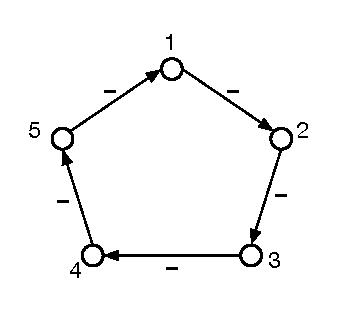
\includegraphics[width=0.45\textwidth]{images/allnegativeC5.eps}}
    	\ \ \ \ 
    	\subfigure[$C_6^{-}$]{\label{fig:d}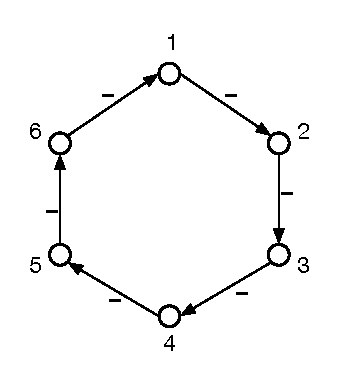
\includegraphics[width=0.45\textwidth]{images/allnegativeC6.eps}}
    	\label{fig:comparison2}
    \end{figure}
\end{frame}

\begin{frame}{Max of $C_5^{-}$ and $C_6^{-}$}
\justifying
    Because of the positive feedback's bound theorem, we know that $\max(G)\leq 2^{\tau^+}$. In both cases, $\tau^+=1$. Moreover, for Aracena's theorem (2008) 
    $C_5^{-}$ doesn't have any fixed point and $C_6^{-}$ has at least two fixed points. Thus
    
    
    \[
        max(C_5^{-}) = 0,
    \]
    
    
    \[
        max(C_6^{-}) \leq 2 \land max(C_6^{-}) \geq 2 \Rightarrow max(C_6^{-}) = 2.
    \]
    
    
\end{frame}

\begin{frame}{Generalization for $C_n$}
    \justifying
    If we consider any $C^+$ and $C^-$ graph, by following the same reasoning as before, we have that $\max(G)\leq 2^{\tau^+}, \forall G \in C_n.$ Then we can consider the following cases:
    \begin{itemize}
        \justifying
        \item if $G \in C_n^-$ with $n$ odd, then $\max(G)=0$ for Aracena's theorem 
        \item if $ G \in C_n^-$ with $n$ even or $G \in C_n^+$, then, knowing that $min(G) \geq 2 \land max(G) \leq 2$ we can deduce that $max(G)=2.$
    \end{itemize}
    
    We can conclude that for any cycle graph the number of fixed points is always below the bound $\binom{n}{\floor{\frac{n}{2}}}.$
\end{frame}

\begin{frame}{$max(K_n^+) \lesseqgtr max(K_n^-)$?}
\justifying
    If we compare $\phi = \binom{n}{\floor{\frac{n}{2}}}$ and $\xi =\frac{2^{n+1}}{n+2},$ for $n \in \mathbb{N}^+:$
    \small{
    \begin{table}
		\begin{tabular}{c|c|c|c}
		$n$ & $\phi = \binom{n}{\floor{\frac{n}{2}}}$ &  $\xi =\frac{2^{n+1}}{n+2}$ & $\phi \geq \xi$ \\\hline
		1 & 1 & 1.3 & $\otimes$\\
		2 & 2 & 2 & \checkmark\\
		3 & 3 & 3.2 & $\otimes$\\
		4 & 6 & 5.3 &\checkmark\\
		5 & 10 & 9.2 &\checkmark\\
		6 & 20 & 16 &\checkmark\\
		7 & 35 & 28.4 & \checkmark\\
		8 & 70 & 51.2 & \checkmark\\
		9 & 126 & 93.1 & \checkmark\\
		10 & 252 & 170.6 & \checkmark\\
		\end{tabular}
	\end{table}
	}
	We can deduce that $\phi \geq \xi,\ \forall n \geq 4.$
\end{frame}

\begin{frame}{Intuition}
\justifying
    Since Richard et al have proved that 
    \begin{itemize}
        \item $\max(K_n^+) \leq \frac{2^{n+1}}{n+2},$
        \item $\max(K_n^-) = \binom{n}{\floor{\frac{n}{2}}},$
    \end{itemize}
    and since $\forall n\geq 4,\ \frac{2^{n+1}}{n+2} \leq \binom{n}{\floor{\frac{n}{2}}},$ we can assert that
    \begin{equation}
        \label{eq:maxKorder}
        \forall n\geq 4,\ \max{K_n^+} \leq \max{K_n^-}.
    \end{equation}
\end{frame}

\begin{frame}{Intuition for $max(K_n)$}
    \justifying
    \begin{exampleblock}{Intuition}
        For all complete signed graph $K_n$, $max(K_n) \leq max(K_n^-)$.
    \end{exampleblock}
    Fix $n \leq 4$. Let $G^{(0)} = K_n^-$. Let $G^{(1)}$ be the graph obtained from $G^{(0)}$ by changing the sign of just one of its edges, such that $G^{(1)}$ has now exactly one edge with positive sign and all others with negative sign.
    
    We assume that this change never implies
    \[
        max(G^{(1)}) > max(G^{(0)}) = max(K_n^-)
    \]
    therefore
    \[
        max(G^{(1)}) \leq max(G^{(0)}) = max(K_n^-)
    \]
\end{frame}

\begin{frame}{Intuition for $max(K_n)$ cont'd}
\justifying
    and so on build $G^{(2)}$, then $G^{(3)}$, $\dots$
    \begin{alignat*}{3}
        max(G^{(2)}) &\leq max(G^{(0)}) &&= max(K_n^-)\\
        max(G^{(3)}) &\leq max(G^{(0)}) &&= max(K_n^-)\\
        &\vdots && \vdots 
    \end{alignat*}
        
    up to $G^{(|E|)} = K_n^+$
    \[
        max(K_n^+) = max(G^{(|E|)}) \leq max(G^{(0)}) = max(K_n^-)
    \]
    that is supported by Inequality \ref{eq:maxKorder}.
\end{frame}

\begin{frame}{Example to Support the Intuition for $max(K_n)$}
    \justifying
    Now we are going to support this intuition through an example for $n=4$.
    \[
        max(G^{(0)}) = max(K_n^-) = \binom{n}{\floor{\frac{n}{2}}} = \binom{4}{2} = \frac{4!}{2!2!} = \frac{24}{4} = 6.
    \]
    
\end{frame}

\begin{frame}{Frame Title}
    \justifying
    \begin{theorem}
    \justifying
    For each complete signed graph of 3 vertices there always exists a positive cycle of size at most 3.
    \end{theorem}
    We know 
    \[
        \forall G,\ max(G) \leq A(n,g^+).
    \]
    In a complete graph ($n \geq 3$) $g^+ = 2$ except for the particular case (we will refer to it with $\star$) in which $\forall v,u \in V\ u,\ \neq v \Rightarrow$ edge $(u,v)$ and $(v,u)$ have different sign. In that case $g^+ = 3$, since it is always possible to consider a subgraph $H$ of $G$ with three vertices and, for the Theorem above, we know that there always exists a cycle of size at most 3 in $H$.
\end{frame}

\begin{frame}{Frame Title}
\justifying
    For $n=4$ we have
    \vspace{-0.5em}
    \begin{alignat*}{3}
        A(n,g^+) &= A(4,2) &&= 6 \text{ or }\\
        A(n,g^+) &= A(4,3) &&= 3 \text{ in $\star$ cases.}
    \end{alignat*}
    It follows that for $n=4$ and $\forall i \in \{0,\dots,|E|\}$ holds
    \[
        max(G^{(i)}) \leq A(4,2) = 6 = max(K_4^-)
    \]
    \hfill $\blacksquare$
\end{frame}

\begin{frame}{Representation of $G^{(0)}$ and $G^{(1)}$}
    \begin{figure}
    	\centering
    	\subfigure[$G^{(0)}$]{\label{fig:a}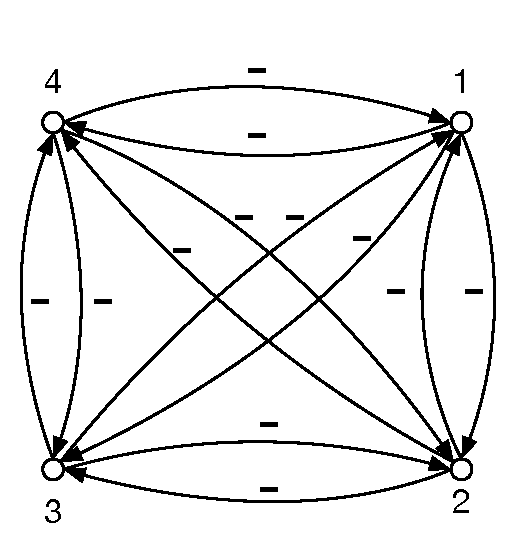
\includegraphics[width=0.45\textwidth]{images/allnegativeK4.eps}}
    	\ \ \ \ 
    	\subfigure[$G^{(1)}$]{\label{fig:b}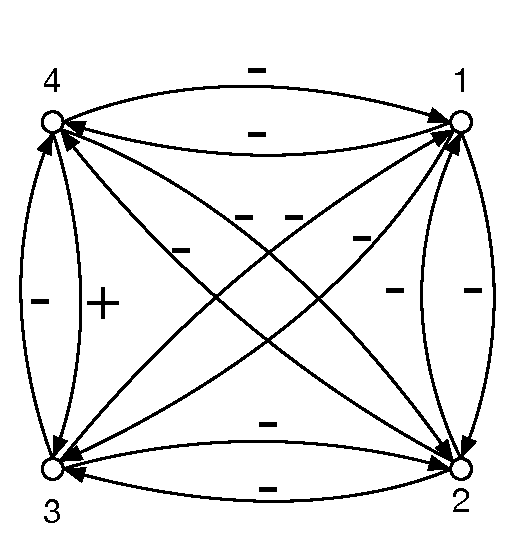
\includegraphics[width=0.45\textwidth]{images/allbut1negativeK4.eps}}
    	\label{fig:comparison}
    \end{figure}
\end{frame}

\begin{frame}{Deduction}
    \justifying
    For each $n \geq 4$ we define the discrete function
    \[
        \psi_n : [n(n-1)] \to C(\psi_n)
    \]
    as
    \[
    \psi_n(x) = \max_{\substack{\forall G = ([n], E) :\\
    |E| = x}} \{ max(G) \}
    \]
    that returns the maximum number of fixed points a graph of $n$ vertices and $x$ edges can have.
\end{frame}

\begin{frame}{Deduction cont'd}
    \begin{block}{Domain of $\psi_n$}
        \justifying
        Let's consider the complete (directed) graph $K_n$, $|E(K_n)| = n(n-1)$, obviously for any directed graph $G$ with $n$ vertices, $n(n-1)$ is an upper bound for $|E|$, therefore there doesn't exist a digraph with $n$ vertices and more than $n(n-1)$ edges. That explains the domain of $\psi_n$.
    \end{block}
    
    \begin{block}{Codomain of $\psi_n$}
    \justifying
        Asserting $C(\psi_n) = [\phi]$ coincides with the Conjecture.
    \end{block}
\end{frame}

\begin{frame}{Deduction cont'd}
    \justifying
    We showed that:
    \begin{itemize}
        \justifying
        \item for $x=n(n-1)$, $\psi_n(x) = \phi$ (demonstrated for $n=4$ and generalized through an intuition to all $n$);
        \item $\forall n \geq 1$, $x=0$, $\psi_n(x) = 1$,;
        \item $\forall n \geq $, $\psi_n(x) \geq 2$; 
    \end{itemize}
    Although emerges clear that for a graph $G=(V,E)$, $max(G)$ is not directly related to $|E|$, we formed the impression that loss of edges for $G$ is not supposed to lead to a gain in fixed points amount, hence we are lead to believe that
    \[
    \argmax_{\forall x \in [n(n-1)]} \{ \psi_n(x) \} = n(n-1)
    \]
\end{frame}

\begin{frame}{Deduction cont'd}
    \justifying
    Considering what we said about complete signed graphs we are also lead to believe that for all sign labellings for $K_n$, we have always
    \[
        max(K_n) \leq max(K_n^-) = \phi
    \]
    therefore
    
    \begin{alertblock}{Deduction}
        \justifying
        $\phi = \binom{n}{\floor{\frac{n}{2}}}$ is an upper bound for the number of fixed points in any signed graph with $n$ vertices.
    \end{alertblock}
\end{frame}
\end{document}